\documentclass[fleqn,letterpaper,12pt,printwatermark=false]{memoir}
% memoir commands to define the text block geometry
\setulmarginsandblock{0.5in}{*}{*}
\setlrmarginsandblock{0.5in}{*}{*}
% put "extra" vertical space at the bottom of a page
\raggedbottom 

\usepackage{amsmath}
\usepackage{etoolbox} % for \ifblank etc
\usepackage{xparse} % for NewDocumentCommand et al.
\usepackage{enumitem}
\usepackage{transparent} % for \transparent, which I use in the watermark
\usepackage[slantedGreek]{mathpazo} \usepackage{helvet} % use Palatino et al.
\usepackage{booktabs} % prettier tables

\usepackage[]{xwatermark}
\newwatermark*[
    allpages,
    color=red!30,angle=45,
    scale=4,
    xpos=-10, ypos=0
]{%
    \transparent{0.4}dhasan example%
}

\usepackage{dashundergaps} % for \gap
\dashundergapssetup{
    teacher-mode=true, % set to true to show answers 
    gap-format=underline,
    teacher-gap-format=underline,
    gap-font={\sffamily},
    gap-numbers=true,
    gap-widen=true,
    gap-extend-percent=150, % note: making this too big might create errors
    gap-number-format=\,\textsuperscript{\normalfont(\thegapnumber)},
}

\usepackage{tcolorbox}
\tcbuselibrary{skins}
\tcbuselibrary{raster}

\usepackage{graphicx}
\graphicspath{ {../images/} }
\begin{document} 

\newcommand{\myClassName}{Pre-AP Algebra 2}
\newcommand{\myUnitNumber}{1}
\newcommand{\myUnitTitle}{Introduction to Functions}
\newcommand{\myLessonNumber}{6}
\newcommand{\myLessonTitle}{Attributes of Linear Functions}


\copypagestyle{myPagestyle}{empty}


\newcommand{\myFooterSize}{\footnotesize}
\makeoddfoot{myPagestyle}{{}}{\myFooterSize{\thepage{}~of~\pageref*{xwmlastpage}}}{\myFooterSize\thetitle}
\makeevenfoot{myPagestyle}{{}}{\myFooterSize{\thepage{}~of~\pageref*{xwmlastpage}}}{\myFooterSize\thetitle}

%
% A command to change the appearance of the cognitive verb 
% in the objectives.
%
\newcommand{\myCognitiveVerb}[1]{\textcolor{blue}{\textbf{#1}}}

%
% Terminology explanation:
%
% "unit" refers to the Algebra 2 unit being taught.
% "section" refers to the section within the unit being taught.
% "heading" refers to the headings in this document (Objectives, Example, ...)
%
\NewDocumentCommand{\myUnitSectionNumberFont}{}{\sffamily\bfseries\HUGE}
\NewDocumentCommand{\myUnitNameFont}{}{\sffamily\large}
\NewDocumentCommand{\mySectionNameFont}{}{\sffamily\bfseries\huge}
\NewDocumentCommand{\myHeadingFont}{}{\sffamily\bfseries\Large}


%
% #1 is the fill-in text
%
\NewDocumentCommand{\myFillInBlank}{m}{%
    \,%
    \gap[u]{#1}%
    \,%
}


% Definition for the LESSON HEADER + OBJECTIVES
%
% #1 : optional unit name
% #2 : optional unit/section number
% #3 : mandatory title
%
\NewDocumentEnvironment{myNotesHeader}{oom}{
    \title{#3}
    \begin{flushleft}
        \IfValueT{#2}{{\myUnitSectionNumberFont#2}}
        \hfill\;\;
        \begin{minipage}[b]{0.75\textwidth}
            \begin{flushright}
                \IfValueT{#1}{
                    {\myUnitNameFont#1}\\ \vspace{0.75em}
                }
                {\mySectionNameFont#3}
            \end{flushright}
        \end{minipage}
        \hrule
    \end{flushleft}
    \noindent{\myHeadingFont Objectives:}
    \begin{enumerate}[label=\arabic*)]
}{
    \end{enumerate}
}


% Definitions related to the VOCABULARY TABLE
%
\newenvironment{myVocabulary}{
    {\noindent{\myHeadingFont Vocabulary:}}\vspace{1em}

    \begin{tabular}{ll}
        \toprule
            \emph{word} & \emph{meaning} \\ 
        \midrule
}{
    \bottomrule
    \end{tabular}
    \vspace{1em}
}

\newcommand{\myVocabularyWord}[2]{%
{\textcolor{blue}{\textbf{#1}}} & #2 \\
}


% Definitions related to an INTRODUCTION
%
\newenvironment{myIntroduction}{
    {\noindent{\myHeadingFont Introduction:}}\vspace{1em}

    \setlength{\leftskip}{3cm}
}{
    \setlength{\leftskip}{0pt}
}


% Definition related to KEY CONCEPTS
%
% #1 : the key concept (which appears as a tcolorbox title)
%
\NewDocumentEnvironment{myKeyConcepts}{ O{Key Concepts:} }{
    \begin{tcolorbox}[
        title=#1, fonttitle=\myHeadingFont,
        coltitle=black, 
        colbacktitle=black!25!yellow, 
        colframe=black!50!yellow,
        colback=white!70!yellow,
        boxrule=2pt, 
        ]
}{
    \end{tcolorbox}
}


% Definition related to EXAMPLES
%
% #1 Optional example number 
% #2 A statement of the example problem.
% #3 How much empty vertical space to leave for the example box.
%
\NewDocumentCommand{\myExample}{omm}{%
    \begin{tcolorbox}[
        enhanced,
        sharp corners, 
        colback=white,
        boxrule=0pt,
        borderline={0.5pt}{0pt}{black,dashed},
        ]
        {\myHeadingFont Example\IfValueT{#1}{{ #1}}:}
        #2
        \tcblower
        \vspace{#3}
    \end{tcolorbox}
}

% Definitions related to PROBLEMS

% A counter to number the problems in the guided notes.
\newcounter{MyProblemCounter}
\setcounter{MyProblemCounter}{1}
\newcommand{\useMyProblemCounter}{\theMyProblemCounter\stepcounter{MyProblemCounter}}

% an environment for two adjacent problems
%
% #1 : directions for all the problems
% #2 : vertical height of the problem boxes
% #3 : details for problem 1
% #4 : details for problem 2
%
\newenvironment{myProblems2}[4]{%
    \noindent
    {\myHeadingFont Practice:}\hspace{0.5em}#1\nopagebreak%
    \begin{tcbraster}[%
        raster equal height,%
        raster columns=2,%
        raster column skip=0.5mm,%
        raster row skip=0.5mm,%
        raster every box/.style={%
            enhanced,%
            sharp corners,%
            colback=white,%
            coltitle=black, colbacktitle=black!10!white,%
            boxrule=0pt, borderline={0.5pt}{0pt}{black},%
            title={\texttt\useMyProblemCounter},%
            },%
        ]%
        \begin{tcolorbox}[attach boxed title to top left]
            #3
            \tcblower\vspace{#2}
        \end{tcolorbox}
        \begin{tcolorbox}[attach boxed title to top right]
            #4
            \tcblower
        \end{tcolorbox}%
}{%
    \end{tcbraster}
}

% an environment for 4 adjacent problems
%
% #1 : directions for all the problems
% #2 : vertical height of the problem boxes
% #3 : details for problem 1
% #4 : details for problem 2
% #5 : details for problem 3
% #6 : details for problem 4
%
\newenvironment{myProblems4}[6]{%
    \noindent
    \textbf{\myHeadingFont Practice:}\hspace{0.5em}#1\nopagebreak%
    \begin{tcbraster}[%
        raster equal height,%
        raster columns=2,%
        raster column skip=0.5mm,%
        raster row skip=0.5mm,%
        raster every box/.style={%
            enhanced,%
            sharp corners,%
            colback=white,%
            coltitle=black, colbacktitle=black!10!white,%
            boxrule=0pt, borderline={0.5pt}{0pt}{black},%
            title={\texttt\useMyProblemCounter},%
            },%
        ]%
        \begin{tcolorbox}[attach boxed title to top left]
            #3
            \tcblower\vspace{#2}
        \end{tcolorbox}
        \begin{tcolorbox}[attach boxed title to top right]
            #4
            \tcblower
        \end{tcolorbox}%
        \begin{tcolorbox}[attach boxed title to bottom left]
            #5
            \tcblower
        \end{tcolorbox}%
        \begin{tcolorbox}[attach boxed title to bottom right]
            #6
            \tcblower
        \end{tcolorbox}%
}{%
    \end{tcbraster}
}
\pagestyle{myPagestyle} 

\checkandfixthelayout
\setlist{labelindent=\parindent,leftmargin=*,itemsep=0.025em,label=$\circ$}

% ---------------------HEADER------------------------------
\begin{myNotesHeader}
    \item \myCognitiveVerb{find} the slope and $y$-intercept of a line from its graph
    \item \myCognitiveVerb{find} the $x$- and $y$-intercepts of a line from its graph
    \item \myCognitiveVerb{find} the slope and intercept of a line from its function, $f(x) = mx+b$.
    \item \myCognitiveVerb{find} the $x$- and $y$-intercepts of a line from its equation
\end{myNotesHeader}

\begin{myVocabulary}
    \myVocabularyWord{slope}
    {
        rate of change, ``rise over run'', change in $y$ divided by change in $x$
    }
    \myVocabularyWord{$x$-intercept}
    {
        the point where the graph crosses the $x$-axis
    }
    \myVocabularyWord{$y$-intercept}
    {
        the point where the graph crosses the $y$-axis
    }
    \myVocabularyWord{linear function}
    {
        a function $f(x)$ with a rule that only has $x$ terms and numbers
    }
    \myVocabularyWord{slope-intercept form}
    {
        a linear function with the rule written as $f(x) = mx+b$
    }
\end{myVocabulary}

% ---------------------CONCEPT 1------------------------------
\begin{myKeyConcepts}[To find $y$-intercept of a line from its graph\dots]
    Follow these steps:
    \setlist{labelindent=\parindent,}
    \begin{enumerate}
        \item \myEmph{Plot}the point where the line crosses the $y$-axis. 
        \item \myEmph{Find}the coordinates of that point. (Let's call them $(x_1,y_1)$.)
        \item $y_1$ is the\myEmph{$y$-coordinate} of the line.
    \end{enumerate}
\end{myKeyConcepts}

\myExample{
    Find the $y$-intercept of this line.
    \begin{center}
        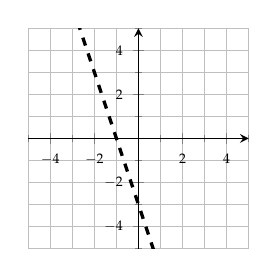
\begin{tikzpicture}
            \begin{axis}[
                width=2in,
                grid=both,
                axis x line = middle,axis y line = middle,
                axis equal image,
                xtick distance = 2, ytick distance = 2, 
                minor tick num = 1,
                xmin = -5, xmax=5,
                ymin = -5, ymax=5,
                tick label style = {font=\tiny},
                ]
                \addplot[dashed,style={line width=1.2pt},no marks, samples=3, domain=-3:4, ] expression { -3*x -3 };
            \end{axis}
        \end{tikzpicture}
    \end{center}
}{1.75in}

It's possible that the line won't cross the $y$-axis exactly at a grid point. 
In that case, if all you have is a graph of the line,
the best you can do is \emph{estimate} the value.

\myExample{
    Find the $y$-intercept of this line. If you need to, estimate its value.
    \begin{center}
        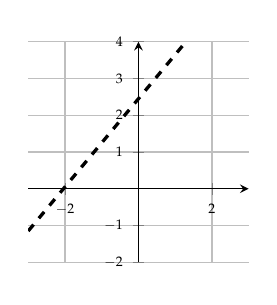
\begin{tikzpicture}
            \begin{axis}[
                width=2in,
                grid=both,
                axis x line = middle,axis y line = middle,
                axis equal image,
                xtick distance = 2, ytick distance = 1, 
                % minor tick num = 1,
                xmin = -3, xmax=3,
                ymin = -2, ymax=4,
                tick label style = {font=\tiny},
                ]
                \addplot[dashed,style={line width=1.2pt},no marks, samples=3, domain=-3:4, ] expression { 1.2*x + 2.45 };
            \end{axis}
        \end{tikzpicture}
    \end{center}
}{2in}

\begin{myKeyConcepts}[To find the slope of a line from its graph\dots]
    Follow these steps:
    \setlist{labelindent=\parindent,}
    \begin{enumerate}
        \item \myEmph{Plot}two points that are on the line. 
        \item \myEmph{Find}the coordinates of both points. Let's call them $(x_1,y_1)$ and $(x_2,y_2)$.
        (Which point is 1 and which is 2 does not matter.)
        \item \myEmph{Calculate} the slope as\myEmph{rise over run}:
        $m = (y_2-y_1)/(x_2-x_1)$.
    \end{enumerate}
\end{myKeyConcepts}

\myExample{
    Find the slope of this line.
    \begin{center}
        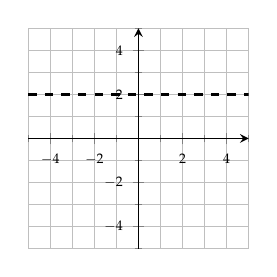
\begin{tikzpicture}
            \begin{axis}[
                width=2.in,
                grid=both,
                axis x line = middle,axis y line = middle,
                axis equal image,
                xtick distance = 2, ytick distance = 2, 
                minor tick num = 1,
                xmin = -5, xmax=5,
                ymin = -5, ymax=5,
                tick label style = {font=\tiny},
                ]
                \addplot[dashed,style={line width=1.2pt}, no marks, samples=3, domain=-5:5, ] expression { 2 };
            \end{axis}
        \end{tikzpicture}
    \end{center}
}{1.25in}

\myExample{
    Find the slope of this line.
    \begin{center}
        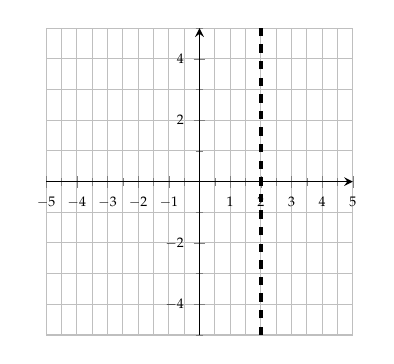
\begin{tikzpicture}
            \begin{axis}[
                width=2.5in,
                grid=both,
                axis x line = middle,axis y line = middle,
                axis equal image,
                xtick distance = 1, ytick distance = 2, 
                minor tick num = 1,
                xmin = -5, xmax=5,
                ymin = -5, ymax=5,
                tick label style = {font=\tiny},
                ]
                \addplot +[mark=none,dashed,style={line width=1.2pt}, black] coordinates {(2, -5) (2, 5)};
            \end{axis}
        \end{tikzpicture}
    \end{center}
}{2in}

\myExample{
    Find the slope of this line.
    \begin{center}
        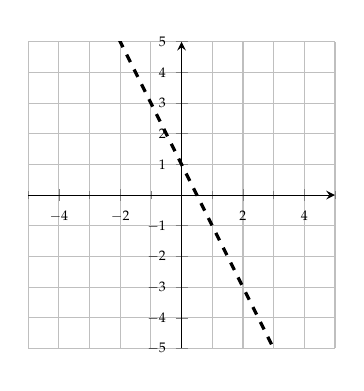
\begin{tikzpicture}
            \begin{axis}[
                width=2.5in,
                grid=both,
                axis x line = middle,axis y line = middle,
                axis equal image,
                xtick distance = 2, ytick distance = 1, 
                minor x tick num = 1,
                xmin = -5, xmax=5,
                ymin = -5, ymax=5,
                tick label style = {font=\tiny},
                ]
                \addplot[dashed,style={line width=1.2pt},no marks, samples=3, domain=-3:4, ] expression { -2*x + 1 };
            \end{axis}
        \end{tikzpicture}
    \end{center}
}{2in}

\begin{myKeyConcepts}[To find the $x$- and $y$-intercepts of a line from its graph\dots]
    Follow these steps:
    \setlist{labelindent=\parindent,}
    \begin{enumerate}
        \item \myEmph{Plot}the points where the line crosses the $x$- and $y$-axes. 
        \item \myEmph{Find}the coordinates of both points. 
        \item The point on the $x$-axis has a $y$-coordinate of 0,
        so its coordinates are $(x,0)$. You may write the\myEmph{$x$-intercept} either as 
        the point $(x,0)$ or just its $x$-coordinate, $x$ as a number.
        \item The point on the $y$-axis has an $x$-coordinate of 0,
        so its coordinates are $(0,y)$. You may write the\myEmph{$y$-intercept} either as 
        the point $(0,y)$ or just its $y$-coordinate, $y$ as a number.
    \end{enumerate}
\end{myKeyConcepts}

\myExample{
    Find $x$- and $y$-intercepts of this line.
    \begin{center}
        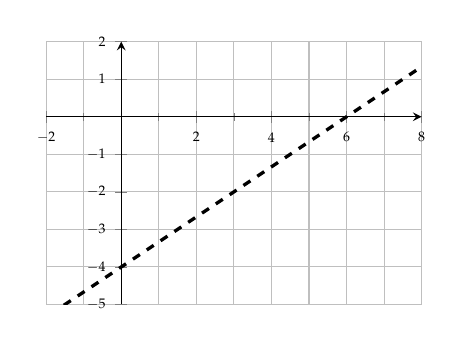
\begin{tikzpicture}
            \begin{axis}[
                width=2.5in,
                grid=both,
                axis x line = middle,axis y line = middle,
                axis equal image,
                xtick distance = 2, ytick distance = 1, 
                minor x tick num = 1,
                xmin = -2, xmax=8,
                ymin = -5, ymax=2,
                tick label style = {font=\tiny},
                ]
                \addplot[dashed,style={line width=1.2pt},no marks, samples=3, domain=-3:10 ] expression { (2/3)*x -4 };
            \end{axis}
        \end{tikzpicture}
    \end{center}
}{1.5in}

\myExample{
    Find $x$- and $y$-intercepts of this line.
    \begin{center}
        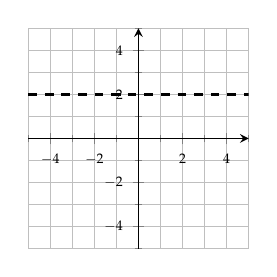
\begin{tikzpicture}
            \begin{axis}[
                width=2.in,
                grid=both,
                axis x line = middle,axis y line = middle,
                axis equal image,
                xtick distance = 2, ytick distance = 2, 
                minor tick num = 1,
                xmin = -5, xmax=5,
                ymin = -5, ymax=5,
                tick label style = {font=\tiny},
                ]
                \addplot[dashed,style={line width=1.2pt}, no marks, samples=100, domain=-5:5, ] expression { 2 };
            \end{axis}
        \end{tikzpicture}
    \end{center}
}{1.2in}

\myExample{
    Find $x$- and $y$-intercepts of this line.
    \begin{center}
        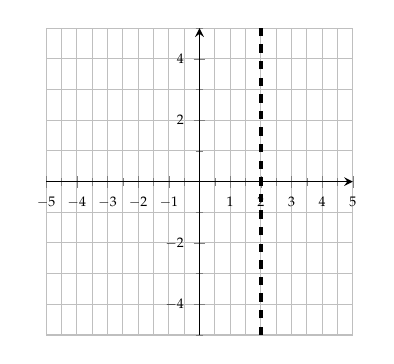
\begin{tikzpicture}
            \begin{axis}[
                width=2.5in,
                grid=both,
                axis x line = middle,axis y line = middle,
                axis equal image,
                xtick distance = 1, ytick distance = 2, 
                minor tick num = 1,
                xmin = -5, xmax=5,
                ymin = -5, ymax=5,
                tick label style = {font=\tiny},
                ]
                \addplot +[mark=none,dashed,style={line width=1.2pt}, black] coordinates {(2, -5) (2, 5)};
            \end{axis}
        \end{tikzpicture}
    \end{center}
}{1.25in}


\begin{myKeyConcepts}[To find the slope and $y$-intercept of a line from the slope-intercept form of its equation\dots]
    Follow these steps:
    \setlist{labelindent=\parindent,}
    \begin{enumerate}
        \item \myEmph{Write down}the slope-intercept form of the equation, $y = mx+b$,
        where $m$ and $b$ are known numbers (not variables).
        \item The \myEmph{slope}is the coefficient ($m$) in front of $x$ in that equation. 
        \item The \myEmph{$y$-intercept}is the number ($b$) in that equation. 
    \end{enumerate}
\end{myKeyConcepts}

It is possible that you know this so well from Algebra 1
that you are wondering why we're talking about it.
If you feel that way, 
make sure that you understand all of the following (yes, simple) examples.
Some of these can be confusing to some students.
Make sure that's not you!

\myExample{
    Find the slope and $y$-intercept of the line corresponding to this function:
    $y = -2x + 4$.
}{1.5in}

\myExample{
    Find the slope and $y$-intercept of the line corresponding to this function:
    $y = -\frac{3}{7}x - \frac{8}{7}$.
}{1.5in}

\myExample{
    Find the slope and $y$-intercept of the line corresponding to this function:
    $y = 6.02x$.
}{1.5in}

\myExample{
    Find the slope and $y$-intercept of the line corresponding to this function:
    $y = x$.
}{1.5in}

\myExample{
    Find the slope and $y$-intercept of the line corresponding to this function:
    $y = 8$.
}{1.5in}



\begin{myKeyConcepts}[To find the intercepts of a line from from its equation\dots]
    Follow these steps:
    \setlist{labelindent=\parindent,}
    \begin{enumerate}
        \item \myEmph{Rewrite}the original equation by substituting $y=0$.
        That will give you an equation involving only $x$.
        \item \myEmph{Solve}that equation for $x$. That solution is the $x$-intercept.
        \item \myEmph{Rewrite}the original equation by substituting $x=0$.
        That will give you an equation involving only $y$.
        \item \myEmph{Solve}that equation for $y$. That solution is the $y$-intercept.
    \end{enumerate}
\end{myKeyConcepts}

It turns out that this method of finding the intercepts\myEmph{works for any equation},
but we're only worried about linear equations for now.
\begin{myLessonBox}[3.5in]
    Find the $x$-intercept by setting $y$ to zero.\par
    Find the $y$-intercept by setting $x$ to zero.
\end{myLessonBox}

\myExample{
    Find the intercepts of the line corresponding to this equation:
    $2x + 3y = 1$.
}{1.5in}

\myExample{
    Find the intercepts of the line corresponding to this equation:
    $2x + 3y = y - 8x + 5$.
}{2in}

\myExample{
    Find the intercepts of the line corresponding to this equation:
    $25y = y + 5$.
}{1.25in}

\myExample{
    Find the intercepts of the line corresponding to this equation:
    $5y = -y$.
}{1.25in}

\myExample{
    Find the intercepts of the line corresponding to this equation:
    $30x = 3x$.
}{1.25in}

\myExample{
    Find the intercepts of the line corresponding to this equation:
    $5x = 5y$.
}{1.25in}

% \begin{myProblems2}%
%     {Factor the following monomials into prime factors.}%
%     {2in}%
%     %
%     {\( 32x^2 \)}
%     {\( 8 x^3y^2z \)}
% \end{myProblems2}
\end{document}